\documentclass[11pt]{amsart}
\usepackage[text={7in,9.5in}]{,geometry}                % See geometry.pdf to learn the layout options. There are lots.
\geometry{letterpaper}                   % ... or a4paper or a5paper or ... 
%\geometry{landscape}                % Activate for for rotated page geometry
%\usepackage[parfill]{parskip}    % Activate to begin paragraphs with an empty line rather than an indent
\usepackage{tikz}
\usetikzlibrary{decorations.pathmorphing}
\usetikzlibrary{decorations.pathreplacing}
\usetikzlibrary{patterns}
\usetikzlibrary{shapes.geometric}
\usepackage{graphicx}
\usepackage{amssymb}
\usepackage{epstopdf}
\DeclareGraphicsRule{.tif}{png}{.png}{`convert #1 `dirname #1`/`basename #1 .tif`.png}

\begin{document}
\begin{enumerate}
\setlength{\itemsep}{5pt}
\setlength{\parskip}{0pt}
\setlength{\parsep}{0pt}
\item [(c)] The closed loop configuration we want to simulate is
\begin{center}
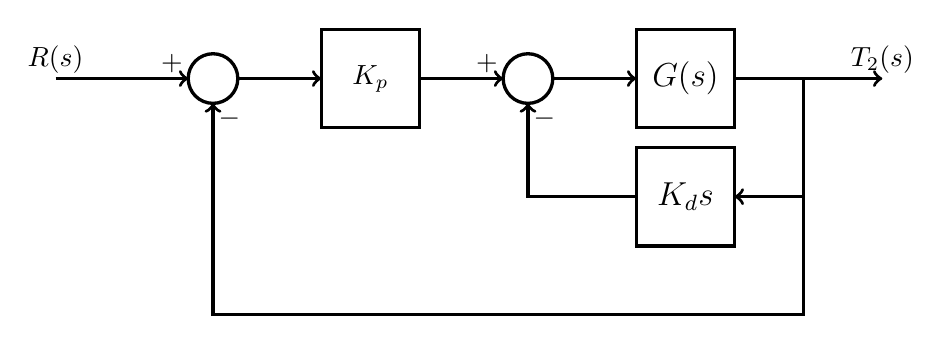
\begin{tikzpicture}[scale=1,inner sep=0pt,outer sep=0pt,very thick,
sysblock/.style={draw,rectangle,inner sep=2pt,minimum width=1.25cm,minimum height=1.25cm,very thick}]
\draw (2,0) node[draw,circle] (sum1) {$\rule{0pt}{18pt}$};
\draw (4,0) node[sysblock] (Kp) {$\large K_p$};
\draw (6,0) node[draw,circle] (sum2) {$\rule{0pt}{18pt}$};
\draw (8,0) node[sysblock] (G) {\large $G(s)$};
\draw (8,-1.5) node[sysblock] (Kd) {\large $K_{d}s$};
\draw[->] (0,0) node[above=2pt] {$R(s)$} -- (sum1.180) node[above left=2pt] {$+$};
\draw[->] (sum1.0) --  (Kp);
\draw[->] (Kp) -- (sum2.180) node[above left=2pt] {$+$};

%\draw[<-] (sum2.90) node[above right=2pt] {$+$} -- (F.-90);
%\draw[<-] (F.90) -- ++(0,1) node[right=2pt] {$T_{a}(s)$};
\draw[->] (sum2) -- (G);
%\draw[->] (Kp.0) -- (G.180);
\draw[->] (G) -- ++(2.5,0) node[above=2pt] {$T_{2}(s)$};
\draw[->] (G) ++(1.5,0) -- ++(0,-1.5) -- (Kd.0);
\draw[->] (G) ++(1.5,0) -- ++(0,-3) -| (sum1.-90) node[below right=2pt] {$-$};
\draw[->] (Kd.180) -| (sum2.-90) node[below right=2pt] {$-$};
\end{tikzpicture}

\end{center}
where $G(s)= \frac{100}{s^{2}+111s+100}$. This has closed loop system
\[
\frac{T_{2}(s)}{R(s)}=T(s)=\frac{100}{s^{2}+(111+100K_d)s+100(1+K_p)},
\]
and using the code
\texttt{\rule{0pt}{0pt}\\
Kp=4.84;\\
Kd=-0.85;\\
\% Configuration \#2
figure(1)\\
T = tf(100*Kp,[1 111+100*Kd 100*(1+Kp)])\\
step(T)}\\
we get the following plot:
\begin{center}
\includegraphics[width=4in]{prob3_1}
\end{center}
This shows that the specifications are met
\end{enumerate}
\end{document}  